\documentclass[../Main.tex]{subfiles}

\begin{document}

\section{Estado del Arte}
La Agencia Espacial Europea ha lanzado dos concursos de optimización anteriormente. El primero tiene relación con un algoritmo de identificación planetaria, el segundo, con la eficiencia de recursos de dicho algoritmo.
\newline \par
En relación a los ángulos de incidencia solar, existe una amplia bibliografía sobre la incidencia solar sobre la superficie terrestre.
\begin{center}
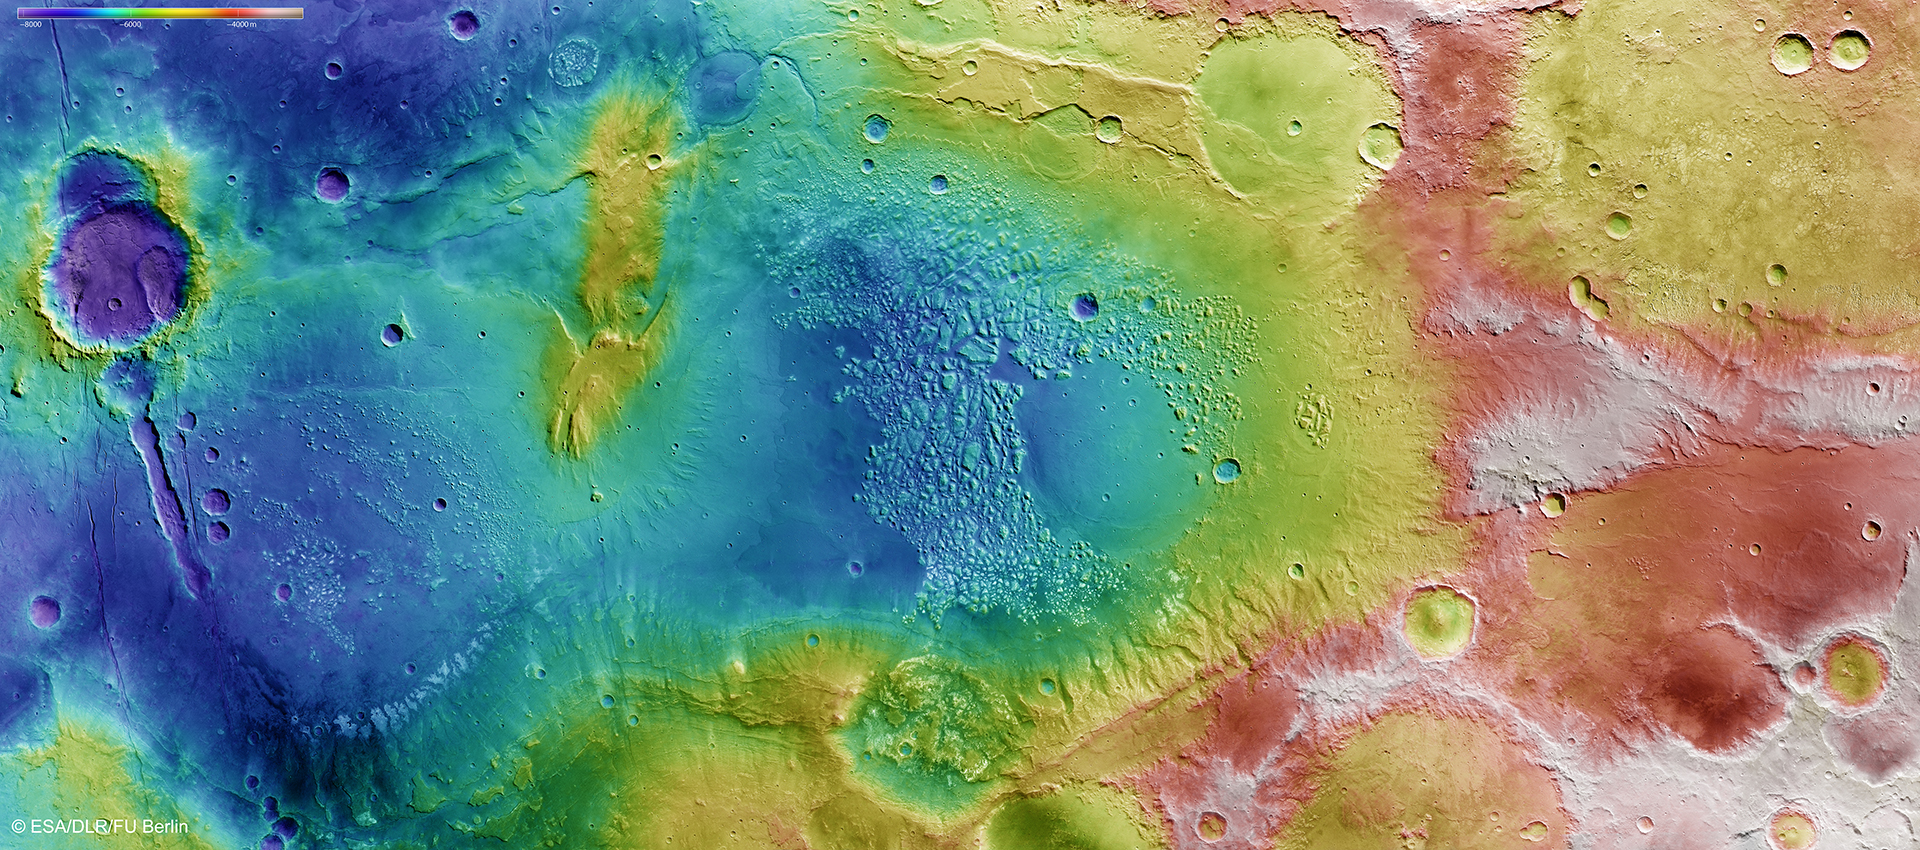
\includegraphics[width=\linewidth, trim={0 10cm 0 0}, clip]{Assets/Ancient_Atlantis.jpg}
\\Figura 1. Imágen con cotas del valle \textit{Ancient Atlantis}
\end{center}

\newline \par
Para el caso de este proyecto, la incidencia debe ser calculada sobre un satelite, por lo que se pueden extender los conceptos anteriores.
\newline \par
Con respecto a la información de los sistemas a bordo de la nave, sus comandos y el funcionamiento de los mismos, es poca la información disponible en la página del concurso. Se prevee que el entendimiento de estos sean de poca relevancia, sin embargo se considera que en la medida enque se profundize sobre los datos, se tenga una mejor comprensión sobre los datos anteriores. 
\end{document}